% Annotated docking-problem figure for the Introduction.
% Image: Gazebo screenshot, BlueROV2 seen from behind on approach with the
% marker-equipped dock ahead. Coordinates are normalised to the image
% (0,0 = bottom left).
\begin{tikzpicture}
  \node[anchor=south west, inner sep=0] (img) {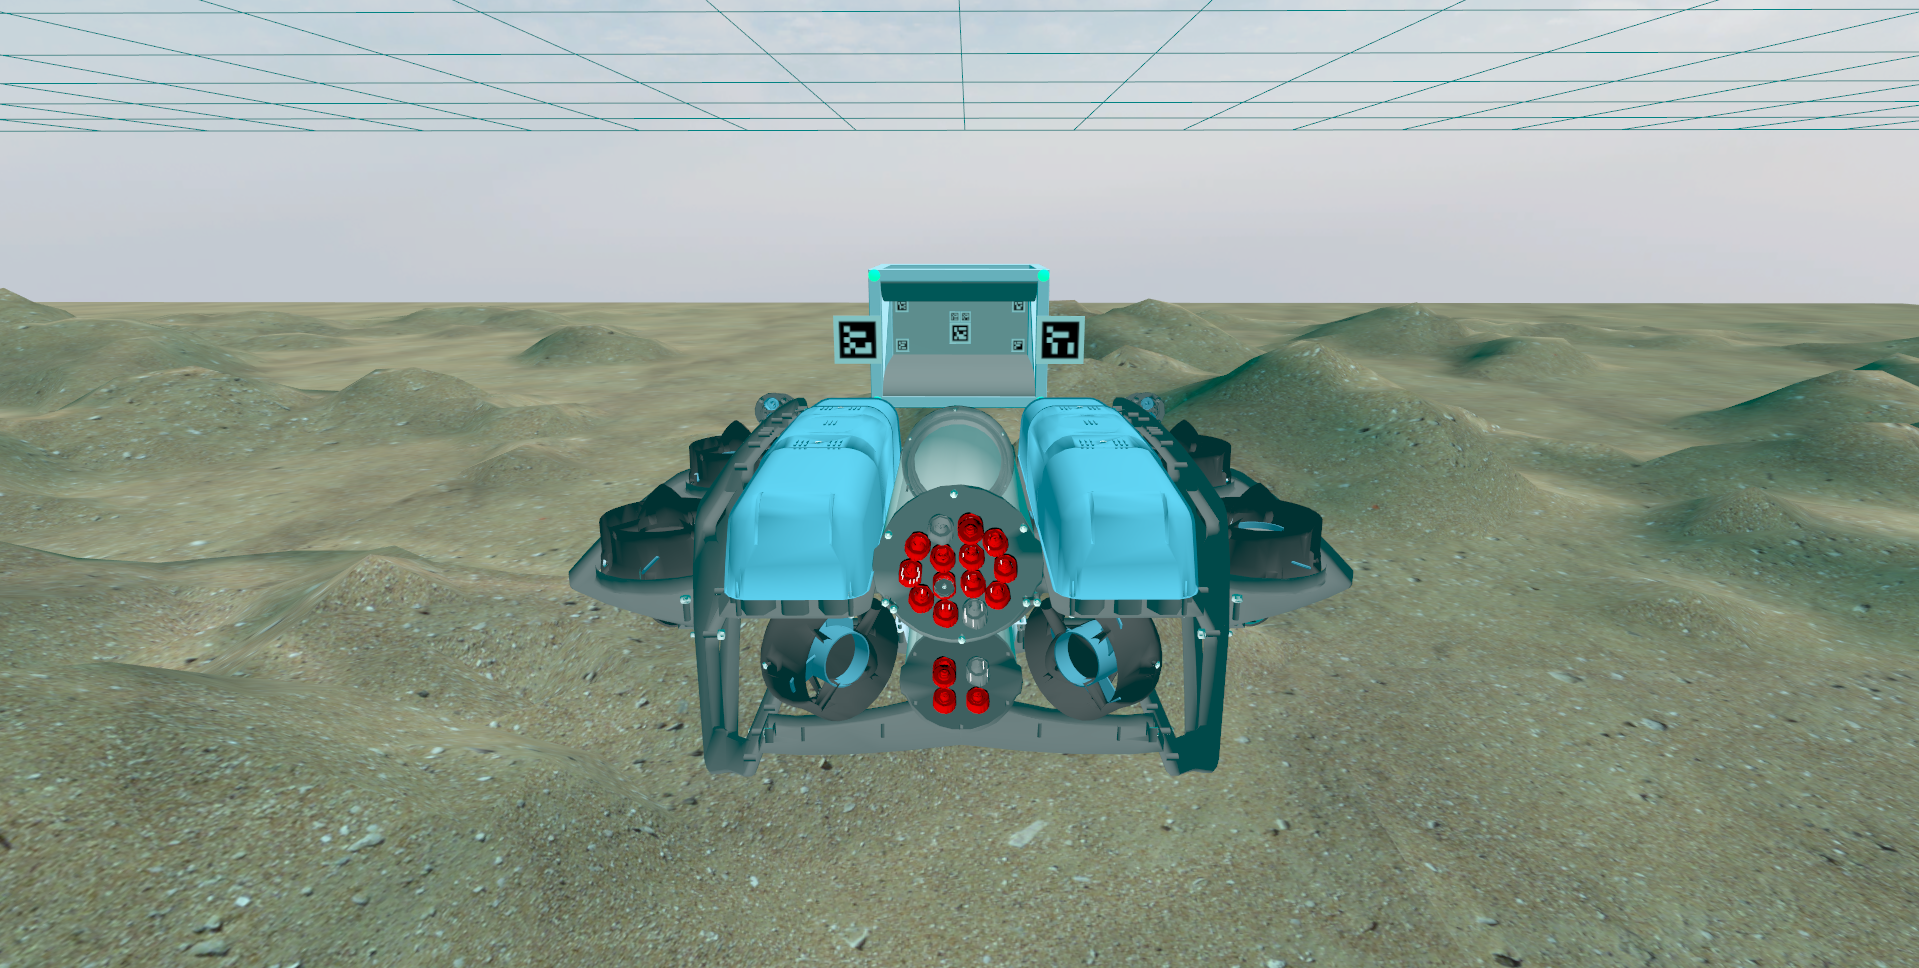
\includegraphics[width=0.85\textwidth]{Images/docking_problem.png}};
  \begin{scope}[x={(img.south east)}, y={(img.north west)},
    lab/.style={font=\scriptsize\bfseries, text=white, align=center, fill=black, fill opacity=0.55,
        text opacity=1, inner sep=3pt, rounded corners=1pt},
    arr/.style={orange, thick, -{Stealth[length=1.6mm]}}]
    \draw[white, thin, dashed, opacity=0.8] (0.50,0.56) -- (0.435,0.635);
    \draw[white, thin, dashed, opacity=0.8] (0.50,0.56) -- (0.565,0.635);
    \node[lab] (lrov) at (0.16,0.55) {BlueROV2\\forward camera};
    \draw[arr] (lrov.east) to[bend right=10] (0.36,0.44);
    \node[lab] (ldock) at (0.83,0.82) {docking station\\passive ArUco markers};
    \draw[arr] (ldock.south) to[bend left=10] (0.575,0.70);
    \node[lab] (lsway) at (0.24,0.82) {wave-driven sway};
    \draw[arr, <->] (0.41,0.77) -- (0.57,0.77);
  \end{scope}
\end{tikzpicture}
